\documentclass[tikz,border=6pt,multi]{standalone}

\usepackage{pgfplots}
\pgfplotsset{compat=1.18}
\usetikzlibrary{
  arrows.meta,
  positioning,
  calc,
  fit,
  backgrounds,
  shapes.geometric,
  shapes.misc
}

\definecolor{emstCore}{RGB}{37,99,235}
\definecolor{emstMarket}{RGB}{5,150,105}
\definecolor{emstSolver}{RGB}{124,58,237}
\definecolor{emstSystem}{RGB}{220,38,38}
\definecolor{emstData}{RGB}{75,85,99}
\definecolor{emstLight}{RGB}{245,247,251}
\definecolor{emstLine}{RGB}{70,78,95}

\tikzset{
  emstbox/.style={
    draw=emstLine,
    rounded corners=2pt,
    very thick,
    align=center,
    minimum height=9mm,
    inner xsep=6pt,
    inner ysep=5pt,
    fill=white,
    font=\sffamily\small
  },
  emstlayer/.style={
    draw=emstLine,
    rounded corners=2pt,
    very thick,
    fill=emstLight,
    inner sep=8pt
  },
  emstarrow/.style={
    -{Latex[length=3mm,width=2mm]},
    very thick,
    draw=emstLine
  },
  emstdashed/.style={
    -{Latex[length=3mm,width=2mm]},
    very thick,
    dashed,
    draw=emstLine
  },
  stage/.style={
    emstbox,
    minimum width=23mm,
    fill=white
  },
  datachip/.style={
    draw=emstData,
    rounded corners=2pt,
    fill=white,
    align=center,
    font=\sffamily\scriptsize,
    inner xsep=4pt,
    inner ysep=3pt
  }
}

% ---------------------------------------------------------------------------
% Figure 1
% ---------------------------------------------------------------------------
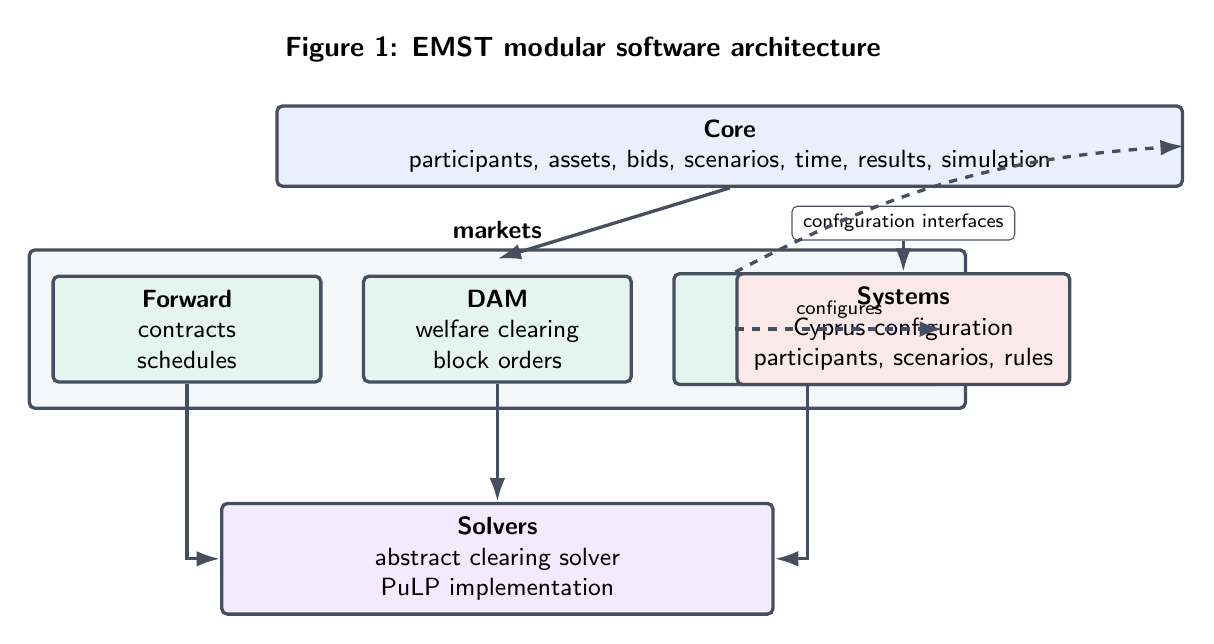
\begin{tikzpicture}[node distance=8mm and 8mm]
  \node[emstbox, fill=emstCore!10, minimum width=115mm] (core)
    {\textbf{Core}\\participants, assets, bids, scenarios, time, results, simulation};

  \node[emstbox, fill=emstMarket!10, below left=11mm and -6mm of core, minimum width=34mm] (fm)
    {\textbf{Forward}\\contracts\\schedules};
  \node[emstbox, fill=emstMarket!10, right=5mm of fm, minimum width=34mm] (dam)
    {\textbf{DAM}\\welfare clearing\\block orders};
  \node[emstbox, fill=emstMarket!10, right=5mm of dam, minimum width=34mm] (ida)
    {\textbf{Intraday}\\IDA1--IDA3\\adjustments};

  \node[emstbox, fill=emstSolver!10, below=15mm of dam, minimum width=70mm] (solver)
    {\textbf{Solvers}\\abstract clearing solver\\PuLP implementation};

  \node[emstbox, fill=emstSystem!10, right=13mm of dam, minimum width=42mm] (cyprus)
    {\textbf{Systems}\\Cyprus configuration\\participants, scenarios, rules};

  \node[datachip, above=4mm of cyprus] (interfaces)
    {configuration interfaces};

  \begin{scope}[on background layer]
    \node[emstlayer, fit=(fm)(dam)(ida), label={[font=\sffamily\small]above:\textbf{markets}}] {};
  \end{scope}

  \draw[emstarrow] (core.south) -- ($(dam.north)+(0,2mm)$);
  \draw[emstarrow] (fm.south) |- (solver.west);
  \draw[emstarrow] (dam.south) -- (solver.north);
  \draw[emstarrow] (ida.south) |- (solver.east);

  \draw[emstdashed] (cyprus.west) -- node[above,font=\sffamily\scriptsize] {configures} (ida.east);
  \draw[emstdashed] (cyprus.north west) to[bend left=12] (core.east);
  \draw[emstdashed] (interfaces.south) -- (cyprus.north);

  \node[font=\sffamily\bfseries, anchor=west] at ($(core.north west)+(0,7mm)$)
    {Figure 1: EMST modular software architecture};
\end{tikzpicture}

% ---------------------------------------------------------------------------
% Figure 2
% ---------------------------------------------------------------------------
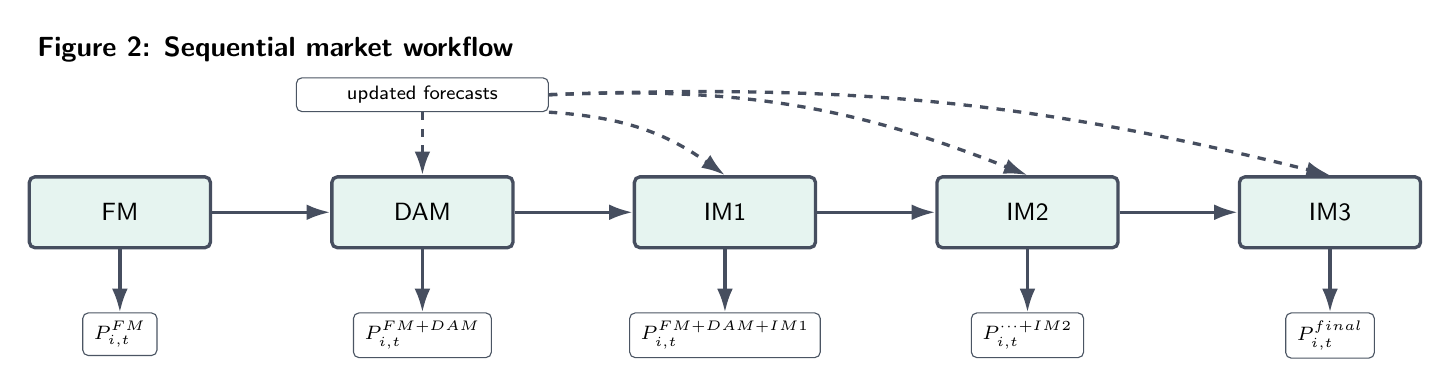
\begin{tikzpicture}[node distance=8mm]
  \node[stage, fill=emstMarket!10] (fm) {FM};
  \node[stage, right=15mm of fm, fill=emstMarket!10] (dam) {DAM};
  \node[stage, right=15mm of dam, fill=emstMarket!10] (im1) {IM1};
  \node[stage, right=15mm of im1, fill=emstMarket!10] (im2) {IM2};
  \node[stage, right=15mm of im2, fill=emstMarket!10] (im3) {IM3};

  \node[datachip, below=8mm of fm] (p0) {$P^{FM}_{i,t}$};
  \node[datachip, below=8mm of dam] (p1) {$P^{FM+DAM}_{i,t}$};
  \node[datachip, below=8mm of im1] (p2) {$P^{FM+DAM+IM1}_{i,t}$};
  \node[datachip, below=8mm of im2] (p3) {$P^{\cdots+IM2}_{i,t}$};
  \node[datachip, below=8mm of im3] (p4) {$P^{final}_{i,t}$};

  \draw[emstarrow] (fm) -- (dam);
  \draw[emstarrow] (dam) -- (im1);
  \draw[emstarrow] (im1) -- (im2);
  \draw[emstarrow] (im2) -- (im3);

  \draw[emstarrow] (fm.south) -- (p0.north);
  \draw[emstarrow] (dam.south) -- (p1.north);
  \draw[emstarrow] (im1.south) -- (p2.north);
  \draw[emstarrow] (im2.south) -- (p3.north);
  \draw[emstarrow] (im3.south) -- (p4.north);

  \node[datachip, above=8mm of dam, minimum width=32mm] (forecasts) {updated forecasts};
  \draw[emstdashed] (forecasts.south) -- (dam.north);
  \draw[emstdashed] (forecasts.south east) to[bend left=16] (im1.north);
  \draw[emstdashed] (forecasts.east) to[bend left=12] (im2.north);
  \draw[emstdashed] (forecasts.east) to[bend left=8] (im3.north);

  \node[font=\sffamily\bfseries, anchor=west] at ($(fm.north west)+(0,16mm)$)
    {Figure 2: Sequential market workflow};
\end{tikzpicture}

% ---------------------------------------------------------------------------
% Figure 3
% ---------------------------------------------------------------------------
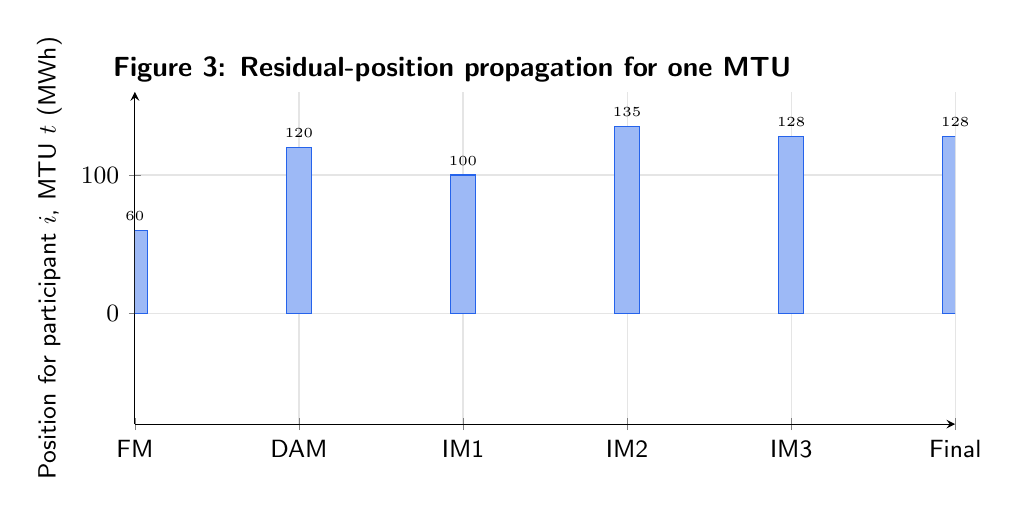
\begin{tikzpicture}
  \begin{axis}[
    width=120mm,
    height=58mm,
    ybar,
    bar width=9pt,
    ymin=-80,
    ymax=160,
    ylabel={Position for participant $i$, MTU $t$ (MWh)},
    symbolic x coords={FM,DAM,IM1,IM2,IM3,Final},
    xtick=data,
    axis lines=left,
    grid=major,
    grid style={draw=gray!20},
    tick label style={font=\sffamily\small},
    label style={font=\sffamily\small},
    nodes near coords,
    every node near coord/.append style={font=\sffamily\tiny},
    title style={font=\sffamily\bfseries}
  ]
    \addplot[fill=emstCore!45, draw=emstCore] coordinates
      {(FM,60) (DAM,120) (IM1,100) (IM2,135) (IM3,128) (Final,128)};
  \end{axis}
  \node[font=\sffamily\bfseries, anchor=west] at (-0.4,4.5)
    {Figure 3: Residual-position propagation for one MTU};
\end{tikzpicture}

% ---------------------------------------------------------------------------
% Figure 4
% ---------------------------------------------------------------------------
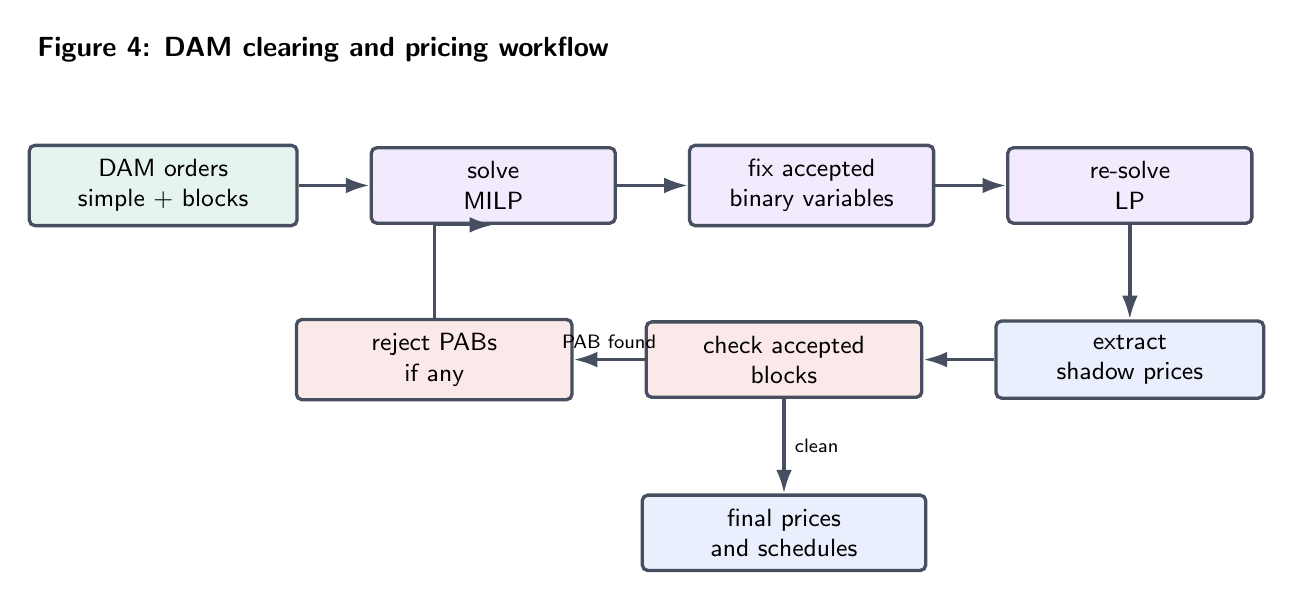
\begin{tikzpicture}[node distance=8mm and 9mm]
  \node[emstbox, fill=emstMarket!10, minimum width=34mm] (input)
    {DAM orders\\simple + blocks};
  \node[emstbox, fill=emstSolver!10, right=of input, minimum width=31mm] (milp)
    {solve\\MILP};
  \node[emstbox, fill=emstSolver!10, right=of milp, minimum width=31mm] (fix)
    {fix accepted\\binary variables};
  \node[emstbox, fill=emstSolver!10, right=of fix, minimum width=31mm] (lp)
    {re-solve\\LP};
  \node[emstbox, fill=emstCore!10, below=12mm of lp, minimum width=34mm] (prices)
    {extract\\shadow prices};
  \node[emstbox, fill=emstSystem!10, left=of prices, minimum width=35mm] (pab)
    {check accepted\\blocks};
  \node[emstbox, fill=emstSystem!10, left=of pab, minimum width=35mm] (reject)
    {reject PABs\\if any};
  \node[emstbox, fill=emstCore!10, below=12mm of pab, minimum width=36mm] (result)
    {final prices\\and schedules};

  \draw[emstarrow] (input) -- (milp);
  \draw[emstarrow] (milp) -- (fix);
  \draw[emstarrow] (fix) -- (lp);
  \draw[emstarrow] (lp) -- (prices);
  \draw[emstarrow] (prices) -- (pab);
  \draw[emstarrow] (pab) -- node[above,font=\sffamily\scriptsize] {PAB found} (reject);
  \draw[emstarrow] (reject.north) |- (milp.south);
  \draw[emstarrow] (pab) -- node[right,font=\sffamily\scriptsize] {clean} (result);

  \node[font=\sffamily\bfseries, anchor=west] at ($(input.north west)+(0,12mm)$)
    {Figure 4: DAM clearing and pricing workflow};
\end{tikzpicture}

% ---------------------------------------------------------------------------
% Figure 5
% ---------------------------------------------------------------------------
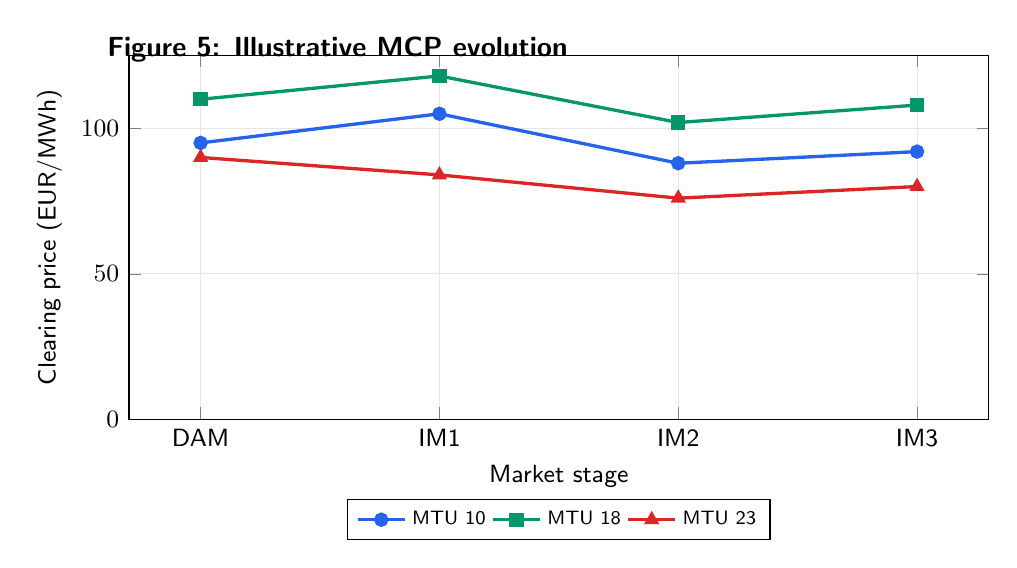
\begin{tikzpicture}
  \begin{axis}[
    width=125mm,
    height=62mm,
    xlabel={Market stage},
    ylabel={Clearing price (EUR/MWh)},
    symbolic x coords={DAM,IM1,IM2,IM3},
    xtick=data,
    ymin=0,
    ymax=125,
    grid=major,
    grid style={draw=gray!20},
    legend style={font=\sffamily\scriptsize, at={(0.5,-0.22)}, anchor=north, legend columns=3},
    tick label style={font=\sffamily\small},
    label style={font=\sffamily\small}
  ]
    \addplot[emstCore, very thick, mark=*] coordinates {(DAM,95) (IM1,105) (IM2,88) (IM3,92)};
    \addlegendentry{MTU 10}
    \addplot[emstMarket, very thick, mark=square*] coordinates {(DAM,110) (IM1,118) (IM2,102) (IM3,108)};
    \addlegendentry{MTU 18}
    \addplot[emstSystem, very thick, mark=triangle*] coordinates {(DAM,90) (IM1,84) (IM2,76) (IM3,80)};
    \addlegendentry{MTU 23}
  \end{axis}
  \node[font=\sffamily\bfseries, anchor=west] at (-0.4,4.7)
    {Figure 5: Illustrative MCP evolution};
\end{tikzpicture}

% ---------------------------------------------------------------------------
% Figure 6
% ---------------------------------------------------------------------------
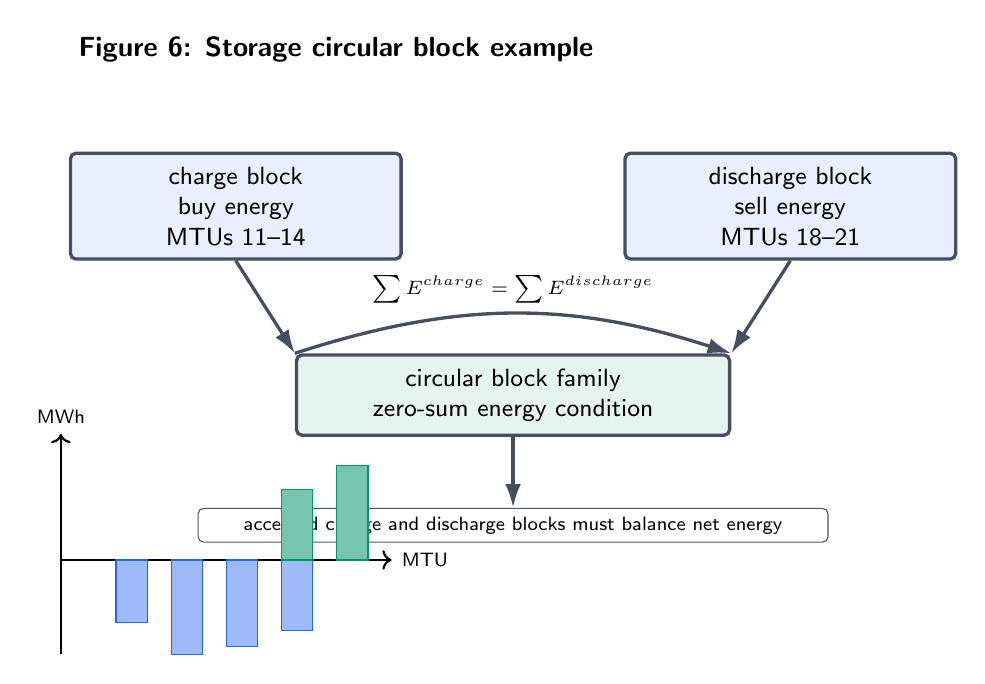
\begin{tikzpicture}[node distance=10mm and 18mm]
  \node[emstbox, fill=emstCore!10, minimum width=42mm] (charge)
    {charge block\\buy energy\\MTUs 11--14};
  \node[emstbox, fill=emstCore!10, right=28mm of charge, minimum width=42mm] (discharge)
    {discharge block\\sell energy\\MTUs 18--21};

  \node[emstbox, fill=emstMarket!10, minimum width=55mm] (family)
    at ($(charge)!0.5!(discharge)+(0,-24mm)$)
    {circular block family\\zero-sum energy condition};

  \draw[emstarrow] (charge.south) -- (family.north west);
  \draw[emstarrow] (discharge.south) -- (family.north east);
  \draw[emstarrow] (family.north west) to[bend left=18] node[above,font=\sffamily\scriptsize] {$\sum E^{charge}=\sum E^{discharge}$} (family.north east);

  \node[datachip, below=9mm of family, minimum width=80mm] (condition)
    {accepted charge and discharge blocks must balance net energy};
  \draw[emstarrow] (family) -- (condition);

  \begin{scope}[shift={($(charge.south west)+(-1mm,-38mm)$)}]
    \draw[->, thick] (0,0) -- (42mm,0) node[right,font=\sffamily\scriptsize] {MTU};
    \draw[->, thick] (0,-12mm) -- (0,16mm) node[above,font=\sffamily\scriptsize] {MWh};
    \foreach \x/\h in {7/0.8,14/1.2,21/1.1,28/0.9} {
      \draw[fill=emstCore!45, draw=emstCore] (\x mm,0) rectangle ++(4mm,-\h cm);
    }
    \foreach \x/\h in {28/0.9,35/1.2} {
      \draw[fill=emstMarket!55, draw=emstMarket] (\x mm,0) rectangle ++(4mm,\h cm);
    }
  \end{scope}

  \node[font=\sffamily\bfseries, anchor=west] at ($(charge.north west)+(0,13mm)$)
    {Figure 6: Storage circular block example};
\end{tikzpicture}
